\graphicspath{{./lab02/Images/}}


\maketitlepage{App Development}{in Android Studio}{Lab 2: Threads}
\maketocpage

\section{Java Threads}
This section offers a brief introduction to threading in Java but anyone with prior knowledge is free to skip to the next section. Note that we are using the Java JDK $8+$ in this part. 

\begin{table}[H]
\center
\begin{tabular}{l|l}
method & functionality \\
\hline
\texttt{Thread(Runnable runnable)} & Creates a new thread \\
\texttt{void start()} & Causes this thread to begin execution \\
\texttt{void join()} & Makes the calling thread wait until this one dies. \\
\texttt{boolean isAlive()} & Returns true iff thread has started and is not dead \\
\texttt{String getName()} & Returns the thread's name
\end{tabular}
\caption{Parts of the Thread API}
\label{table:tapi}
\end{table}

Threads, in its simplest form, are a way to execute two (or more) blocks of code at the same time while sharing certain resources. Each thread executes a run method, line by line, and once started, we have limited control over the order of which thread is being executed\footnote{A context switch is when an operating system switches execution from one thread to another}. In listing \ref{listing:tord} we have three threads, the thread that starts the other two (the main thread) which will print \texttt{X} and \texttt{thread1} and \texttt{thread2}, printing \texttt{A} and \texttt{1} respectively. Running this program produces an nondeterministic output, in fact all possible permutations of \texttt{A}, \texttt{1} and \texttt{X} can be printed.

\begin{lstlisting}[style=A_Java, caption={Order of thread execution}, label={listing:tord}]
public static void main(String[] args) {
    Thread thread1 = new Thread(() -> System.out.print("A"));
    Thread thread2 = new Thread(() -> System.out.print("1"));
    thread1.start();
    thread2.start();
    System.out.print("X");
}
\end{lstlisting}

One reason to use threads is to keep an UI from locking while a long task is happening in the background. Listing \ref{listing:infoui} starts a thread and keeps the user informed that the background job is still running. A more familiar version of this idea is a spinning wheel for the user to look at while he waits.

\begin{lstlisting}[style=A_Java, caption={UI keeping user informed on progress}, label={listing:infoui}]
public class Main {
    public static void main(String[] args) {
        try {
            Thread carpenter = new Thread(() -> buildHouse(3));
            System.out.println("Ready to work");
            carpenter.start();
            while (true) {
                System.out.println("Work in progress...");
                carpenter.join(500);
                if (carpenter.isAlive()) continue;
                System.out.println("Work complete");
                break;
            }
        } catch (InterruptedException ex) {
            ex.printStackTrace();
        }
    }
    public static void buildHouse(int sec) {
        long timePoint = System.currentTimeMillis() + sec * 1000;
        while(System.currentTimeMillis() < timePoint); // loop for sec seconds
    }
}
\end{lstlisting}

A race conditions can occur when two threads access and edit the same resource in an unexpected order. Suppose thread A and B are both running and their job is to increment a shared variable X, which is set as 0. Thread A loads the value of X as 0 into registry when a context switch occurs and thread B loads the value of X into registry as 0 too, then B adds one and stores the value in X before another context switch when thread A does the same, both adding 1 to 1, so the variable ends up as 1, not 2. The part of the code where race conditions can occur is called a critical section. We must pay close attention to them when dealing with threads.\\

In listing \ref{listing:rcon} we start a thousand threads that increment two variables which are initially equal and then check if they are still equal, upon which they increment a counter. A sequential run of such a program would always increment the variable but what can happen here is that thread $i$ is running and has just incremented the variable \texttt{a} when a context switch occurs and thread $j$ starts to run which now increments \texttt{a} again and then \texttt{b} and when done, checks if they are equal which they are not since thread $i$ only incremented \texttt{a} so $j$ will not increment the counter variable. Of course we can get lucky and everything happens in the correct order, even most of the time, but a slim chance of a race condition is all that is needed to make an entire program ruined.  

\begin{lstlisting}[style=A_Java, caption={Race condition}, label={listing:rcon}]
public class Main {
    private static int counter = 0, a = 0, b = 0;
    public static void main(String[] args) {
        try {
            Thread[] threads = new Thread[1000];
            for (int i = 0; i < threads.length; i++) {
                threads[i] = new Thread(() -> {
                    if (++a == ++b) counter++;
                });
                threads[i].start();
            }
            for (Thread t : threads) t.join();
            System.out.println(counter);
        } catch (InterruptedException e) {
            e.printStackTrace();
        }
    }
}
\end{lstlisting}

To deal with race conditions, we can identify the critical section and make sure that only one thread can operate there at any given time. That does however come at the cost of execution speed so we must place such lockouts wisely. When some thread arrives at a critical section, it should either be locked and make the thread wait or as soon as the thread 'steps in', the section should lock other threads out, until the current one is done. This can be done with the Java keyword \verb!synchronized!. Synchronized methods can only be run by one thread at a time. Another approach is to use a mutex. One can think of a mutex like a single key which you must acquire to reach a critical section but once used, no one else can use it until the current key user has returned it after leaving the critical section. In Java, mutexes are instances of the class \texttt{Semaphore}, a more general case of a mutex for arbitrary number of keys (even a negative amount!). Using a Semaphore initialized with a key count of 1, the following mutex will fix our race condition.

\begin{lstlisting}[style=A_Java]
threads[i] = new Thread(() -> {
  try {
    mutex.acquire();                    // Get the only key
    /* Critical section begins */
    if (++a == ++b) counter++;
    /* Critical section ends */
    mutex.release();                    // Give back the only key
  } catch (InterruptedException e) {
    e.printStackTrace();
  }
});
\end{lstlisting}

Using such locks brings about another problem. What if Thread $i$ is waiting on thread $j$ and thread $j$ is waiting on thread $i$? That will go on forever and is called a deadlock. Taking a look at listing \ref{listing:dlock}, suppose that the thread \texttt{t1} start and acquires \texttt{mutex1} but as soon as he has, a context switch occurs and the thread \texttt{t2} starts to run and acquires \texttt{mutex2}. Now it does not matter which thread is running, both mutexes are locked and both threads are unable to acquire the 'key'.

\begin{lstlisting}[style=A_Java, caption={Deadlock}, label={listing:dlock}]
public static void main(String[] args) {
    Semaphore mutex1 = new Semaphore(1);
    Semaphore mutex2 = new Semaphore(1);
    Thread t1 = new Thread(() -> {
        try {
            mutex1.acquire();
            mutex2.acquire();
            mutex1.release();
            mutex2.release();
        } catch (InterruptedException e) {
            e.printStackTrace();
        }
    });
    Thread t2 = new Thread(() -> {
        try {
            mutex2.acquire();
            mutex1.acquire();
            mutex2.release();
            mutex1.release();
        } catch (InterruptedException e) {
            e.printStackTrace();
        }
    });
}
\end{lstlisting}

Thread pools are used to gain more control over threads in Java. We can control the upper bound of how many threads are active at any given time from a pool. This is done with \texttt{Executor} and \texttt{ExecutorService}. In listing \ref{listing:thpool} we have a thread pool with a thread limit of five but 15 threads to start. As soon as 5 threads are already active, no more are added until at least one of them finishes.

\begin{lstlisting}[style=A_Java, caption={Thread pool}, label={listing:thpool}]
public static void main(String[] args) {
    ExecutorService executor = Executors.newFixedThreadPool(5);
    for (int i = 0; i < 15; i++) {
        executor.execute(() -> {
            try {
                System.out.println(Thread.currentThread().getName() + ": Hi");
                Thread.sleep(1000);
                System.out.println(Thread.currentThread().getName() + ": Bye");
            } catch (InterruptedException e) {
                e.printStackTrace();
            }/
        });
    }
    executor.shutdown();
}
\end{lstlisting}

\section{The Android UI thread}
Upon starting an Android app, thread is created to which will run our launcher activity and from there on, any component (which we will look at later) started. It also handles all events and interaction concerning the UI. No other threads should interact directly with the UI. This thread is called the main thread or the UI thread.\\

Suppose our app needs to run a long and expansive task, taking 10 seconds to execute. If we were to run that on the main thread, then it would become not be able to listen for any events and the UI would essentially be locked and eventually the operating system would warn the user that the app is not responding. To avoid this, all expansive tasks should be performed by new threads in the background of the main one. Tasks like calling a web server, downloading and many more.\\

Just as the UI thread shouldn't run long tasks, the vice versa holds, that long task running threads should never update the UI. The two rules of thumb are
\begin{itemize}
\item \textbf{Never run a long task on the UI thread}
\item \textbf{Never update your UI from any thread other than the UI thread}
\end{itemize}

There are multiple Android specific ways to create and managing threads but we will only look at few here.

\section{Asynchronous tasks}
The abstract class \texttt{AsyncTask} provides an easy way to perform a background task which can talk to the UI thread. Asynchronous tasks are used for a short task required to run in a background thread, preferably not running longer than a few seconds. They are however bound to the lifetime of their activity.\\

The \texttt{AsyncTask} class has 3 generic types,
\begin{itemize}
\item \texttt{Params}. The type of parameter sent to task upon execution.
\item \texttt{Progress}. The type of progress unit published during task.
\item \texttt{Result} The type of result returned by the task.
\end{itemize}
All of these can be of the type \texttt{Void} which will omit that type from the task. Asynchronous tasks also has 4 stages,
\begin{itemize}
\item \texttt{onPreExecute}. Runs on the UI thread before task is executed. Used as a initializer for the background task.
\item \texttt{doInBackground}. Runs on a separate thread, performing the actual task, publishing progress and returning the result.
\item \texttt{onProgressUpdate}. Runs on the UI thread where receives progress updates from the background task.
\item \texttt{onPostExecute}. Runs on the UI thread where it processes the result of the background task once done.
\end{itemize}
Additionally \texttt{onCancel} is called if the tasked is canceled instead of \texttt{onPostExecute}. The cancellation should be done by the UI thread but once canceled, the \texttt{doInBackground} method will not stop unless it regularly checks if the task has been canceled.\\

Asynchronous task should always be created and started by the UI thread. To start a asynchronous task, we can call \texttt{execute} or \texttt{executeOnExecutor}, the latter when using a Thread pool. To communicate with the UI thread we must either declare our task class (that inhertis from \texttt{AsyncTask}) as a subclass of our activity or use a callback interface.

\begin{lstlisting}[style=A_XML, caption={Layout for AsyncTask program}, label={listing:asynlay}]
<?xml version="1.0" encoding="utf-8"?>
<LinearLayout xmlns:android="http://schemas.android.com/apk/res/android"
    xmlns:tools="http://schemas.android.com/tools"
    android:layout_width="match_parent"
    android:layout_height="match_parent"
    android:orientation="vertical"
    android:gravity="center"
    tools:context="com.ru.droid.lab.MainActivity">
    <Button
        android:id="@+id/btn_start"
        android:layout_width="wrap_content"
        android:layout_height="wrap_content"
        android:text="Start thread"/> <!-- Move to res/strings -->
    <Button
        android:id="@+id/btn_cancel"
        android:layout_width="wrap_content"
        android:layout_height="wrap_content"
        android:text="Cancel thread"/> <!-- Move to res/strings -->
    <TextView
        android:id="@+id/msg"
        android:layout_width="wrap_content"
        android:layout_height="wrap_content"
        android:text="Idle"/> <!-- Move to res/strings -->
    <ProgressBar
        android:id="@+id/prog"
        style="?android:attr/progressBarStyleHorizontal"
        android:layout_width="match_parent"
        android:layout_height="wrap_content"
        android:layout_margin="15dp"
        android:visibility="invisible"
        android:max="1000"/>
</LinearLayout>
\end{lstlisting}

\begin{lstlisting}[style=A_Java, caption={Background task done with asynchronous task}, label={listing:asyncprog}]
public class MainActivity extends AppCompatActivity {

    private ProgressBar progressBar;
    private TextView message;
    private MyTask task;

    @Override
    protected void onCreate(Bundle savedInstanceState) {
        super.onCreate(savedInstanceState);
        setContentView(R.layout.activity_main);

        progressBar = (ProgressBar)findViewById(R.id.prog);
        message = (TextView)findViewById(R.id.msg);

        findViewById(R.id.btn_start).setOnClickListener(new View.OnClickListener() {
            @Override
            public void onClick(View v) {
                if (task == null || task.getStatus() != AsyncTask.Status.RUNNING) {
                    task = new MyTask();
                    task.execute(5);
                }
            }
        });

        findViewById(R.id.btn_cancel).setOnClickListener(new View.OnClickListener() {
            @Override
            public void onClick(View v) {
                if (task != null && task.getStatus() == AsyncTask.Status.RUNNING) {
                    task.cancel(true);
                }
            }
        });
    }

    public class MyTask extends AsyncTask<Integer /* Params */, 
            Integer /* Progress */, Void /* Result */> {
            
        @Override
        protected void onPreExecute() {
            progressBar.setVisibility(View.VISIBLE);
            progressBar.setProgress(0);
            message.setText("Running"); // should be a resource string!
        }
        
        @Override
        protected Void doInBackground(Integer... params) {
            long startTime = System.currentTimeMillis();
            long endTime = params[0] * 1000 + startTime;
            long timeInterval = endTime - startTime;
            long timeNow;
            int last = 0;
            // Run for params[0] seconds given that the task has not been canceled.
            while (!this.isCancelled() && 
                    (timeNow = System.currentTimeMillis()) < endTime) {
                // Calculate ratio
                int progress = (int)(1000 * (timeNow - startTime) 
                        / (double)timeInterval);
                // Send progress update if it has changed
                if (progress != last) {
                    last = progress;
                    publishProgress(progress);
                }
            }
            return null; // return null with Void result
        }

        @Override
        protected void onPostExecute(Void results) {
            message.setText("Complete"); // should be a resource string!
            taskCleanUp();
        }

        @Override
        protected void onCancelled() {
            message.setText("Cancelled"); // should be a resource string!
            taskCleanUp();
        }

        @Override
        protected void onProgressUpdate(Integer... values) {
            progressBar.setProgress(values[0]);
        }
    }

    private void taskCleanUp() {
        task = null;
        progressBar.setVisibility(View.INVISIBLE);
    }
}
\end{lstlisting}

\section{Loopers and Handlers}
A looper provides a thread with a message queue (message being some data or job to process) and keeps checking if any data to process. Each thread can only have one looper but does not need to have one. The UI thread uses this mechanic to process events. Messages are handled by handlers. Each thread can have many handlers. Handlers are bound to a single thread that must have a Looper (and therefore, a message queue) and can post data to a Looper's message queue or process it. Handlers can add a message to the message queue in a thread from another thread that will be processed eventually. A handler can therefore easily communicate with the UI thread from another thread.

\begin{figure}[H]
\centering
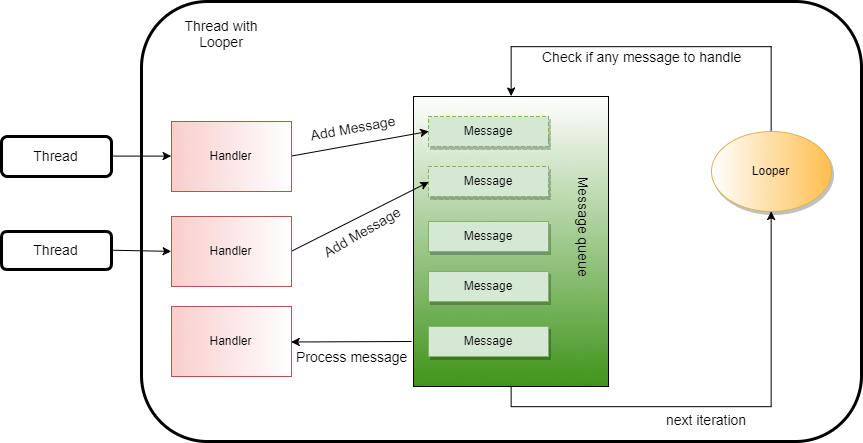
\includegraphics[scale=0.5]{looper.png}
\caption{Simple calculator}
\label{fig:simcal}
\end{figure}

\begin{lstlisting}[style=A_XML,caption={Layout for handler program},label={listing:switchlayout}]
<?xml version="1.0" encoding="utf-8"?>
<LinearLayout xmlns:android="http://schemas.android.com/apk/res/android"
    xmlns:tools="http://schemas.android.com/tools"
    android:layout_width="match_parent"
    android:layout_height="match_parent"
    android:orientation="vertical"
    android:gravity="center"
    tools:context="com.ru.droid.lab.MainActivity">
    <Switch
        android:id="@+id/thread_switch"
        android:layout_width="wrap_content"
        android:layout_height="wrap_content" />
    <ProgressBar
        android:id="@+id/prog"
        style="?android:attr/progressBarStyle"
        android:layout_width="wrap_content"
        android:layout_height="wrap_content"
        android:visibility="invisible" />
</LinearLayout>
\end{lstlisting}

\begin{lstlisting}[style=A_Java, caption={Background job with a thread and communication to UI thread with a handler}, label={listing:layoutprg}]
public class MainActivity extends AppCompatActivity {
    @Override
    protected void onCreate(Bundle savedInstanceState) {
        super.onCreate(savedInstanceState);
        setContentView(R.layout.activity_main);
        final Handler handler = new Handler(Looper.getMainLooper());
        final ProgressBar progressBar = (ProgressBar)findViewById(R.id.prog);
        final Switch aSwitch = (Switch)findViewById(R.id.thread_switch);
        aSwitch.setOnCheckedChangeListener(
                new CompoundButton.OnCheckedChangeListener() {
            @Override
            public void onCheckedChanged(
                    CompoundButton buttonView, boolean isChecked) {
                if (isChecked) {
                    Thread backgroundThread = new Thread(new Runnable() {
                        @Override
                        public void run() {
                            // Make UI thread run the given runnable
                            handler.post(new Runnable() {
                                @Override
                                public void run() {
                                    aSwitch.setClickable(false);
                                    progressBar.setVisibility(View.VISIBLE);
                                }
                            });
                            // Wait 5000 ms on backgroundThread
                            SystemClock.sleep(5000);
                            // Make UI thread run the given runnable
                            handler.post(new Runnable() {
                                @Override
                                public void run() {
                                    progressBar.setVisibility(View.INVISIBLE);
                                    aSwitch.setClickable(true);
                                    aSwitch.setChecked(false);
                                }
                            });
                        }
                    });
                    backgroundThread.start();
                }
            }
        });
    }
}
\end{lstlisting}

\section{RxAndroid}
{\Huge TODO(find some assignment...)}
Write chapter
(3rd party option for threading)

\begin{lstlisting}[style=A_XML]
<?xml version="1.0" encoding="utf-8"?>
<LinearLayout xmlns:android="http://schemas.android.com/apk/res/android"
    xmlns:tools="http://schemas.android.com/tools"
    android:layout_width="match_parent"
    android:layout_height="match_parent"
    android:orientation="vertical"
    android:gravity="center"
    tools:context="com.ru.droid.lab.MainActivity">

    <ProgressBar
        android:id="@+id/progress"
        style="?android:attr/progressBarStyle"
        android:layout_width="wrap_content"
        android:layout_height="wrap_content"
        android:visibility="invisible" />

    <TextView
        android:id="@+id/text"
        android:layout_width="wrap_content"
        android:layout_height="wrap_content" />
    <Button
        android:id="@+id/button"
        android:layout_width="wrap_content"
        android:layout_height="wrap_content"
        android:text="click me"/>
</LinearLayout>
\end{lstlisting}

\begin{lstlisting}[style=A_Java]
public class MainActivity extends AppCompatActivity {

    private TextView textView;
    private ProgressBar progress;
    private Button button;
    private Observable<String> fetchData = Observable.fromCallable(new Callable<String>() {

        private boolean returnSwap = false;

        @Override
        public String call() throws Exception {
            SystemClock.sleep(2500);
            return (returnSwap = !returnSwap) ? "A" : "B";
        }
    }).subscribeOn(Schedulers.io()).observeOn(AndroidSchedulers.mainThread());
    private Observer<String> displayData = new Observer<String>() {
        @Override
        public void onSubscribe(@NonNull Disposable d) {
            progress.setVisibility(View.VISIBLE);
        }

        @Override
        public void onNext(@NonNull String s) {
            textView.setText(s);
        }

        @Override
        public void onError(@NonNull Throwable e) {
            Toast.makeText(MainActivity.this, "Download failed", Toast.LENGTH_SHORT).show();
            textView.setText("Error");
            progress.setVisibility(View.INVISIBLE);
        }

        @Override
        public void onComplete() {
            Toast.makeText(MainActivity.this, "Download complete", Toast.LENGTH_SHORT).show();
            progress.setVisibility(View.INVISIBLE);
            button.setClickable(true);
        }
    };

    @Override
    protected void onCreate(Bundle savedInstanceState) {
        super.onCreate(savedInstanceState);
        setContentView(R.layout.activity_main);

        textView = (TextView)findViewById(R.id.text);
        progress = (ProgressBar)findViewById(R.id.progress);
        button = (Button)findViewById(R.id.button);

        findViewById(R.id.button).setOnClickListener(new View.OnClickListener() {
            @Override
            public void onClick(View v) {
                button.setClickable(false);
                fetchData.subscribe(displayData);
            }
        });
    }
}
\end{lstlisting}

\section{Assignment - Bouncing ball}
{\Huge TODO(find some assignment...)}
Something using primitive graphics that moves it in a background thread.... like moving a ball around the phone...



\begin{lstlisting}[style=A_XML]
<?xml version="1.0" encoding="utf-8"?>
<LinearLayout xmlns:android="http://schemas.android.com/apk/res/android"
    xmlns:tools="http://schemas.android.com/tools"
    android:layout_width="match_parent"
    android:layout_height="match_parent"
    android:orientation="vertical"
    android:gravity="center"
    tools:context="com.ru.droid.lab.MainActivity">
    <com.ru.droid.lab.GraphicView
        android:id="@+id/canvas"
        android:layout_height="match_parent"
        android:layout_width="match_parent"/>
</LinearLayout>
\end{lstlisting}
\begin{lstlisting}[style=A_Java]
public class Circle {
    private float x;
    private float y;
    private float radius;
    private float horizontalSpeed;
    private float verticalSpeed;

    private static Circle main;
    public static Circle getCircle() {
        if (main == null) main = new Circle();
        return main;
    }

    public Circle() {
        x = 150;
        y = 250;
        radius = 50;
        // You can edit the movement speed here
        horizontalSpeed = 0.01f;
        verticalSpeed = 0.01f;
    }

    public void update() {
        x += horizontalSpeed;
        y += verticalSpeed;
    }

    public void changeHorizontalDirection() {
        horizontalSpeed = -horizontalSpeed;
    }

    public void changeVerticalDirection() {
        verticalSpeed = -verticalSpeed;
    }

    public boolean positiveHorizontalDirection() {
        return horizontalSpeed > 0;
    }

    public boolean positiveVerticalDirection() {
        return verticalSpeed > 0;
    }

    public float getX() {
        return this.x;
    }

    public float getY() {
        return this.y;
    }

    public float getRadius() {
        return this.radius;
    }
}
\end{lstlisting}
\begin{lstlisting}[style=A_Java]
public class GraphicView extends View {

    private Paint paint;

    public GraphicView(Context context, @Nullable AttributeSet attrs) {
        super(context, attrs);
        paint = new Paint();
        paint.setARGB(255, 0, 255, 0); // (alpha, red, green, blue)
        paint.setStyle(Paint.Style.FILL_AND_STROKE);
    }

    @Override
    public void onDraw(Canvas canvas) {
        canvas.drawCircle(Circle.getCircle().getX(), Circle.getCircle().getY(), 
                Circle.getCircle().getRadius(), paint);
    }

    public void update() {
        this.invalidate(); // forces a redraw
    }
}
\end{lstlisting}
\begin{lstlisting}[style=A_Java]
public class MainActivity extends AppCompatActivity {

    private GraphicView canvas;

    @Override
    protected void onCreate(Bundle savedInstanceState) {
        super.onCreate(savedInstanceState);
        setContentView(R.layout.activity_main);
        canvas = (GraphicView)findViewById(R.id.canvas);

        // TODO
        // Use another thread to continuously update the circle's position
        // Update the view from the UI thread
        // The ball should bounce on boundaries and must not leave the view
        // You can use canvas.getWidth() and canvas.getHeight() for borders
    }
}
\end{lstlisting}


